\documentclass[border=10pt]{standalone}
\usepackage{tikz}
\usetikzlibrary{arrows.meta, shapes, calc}

\begin{document}

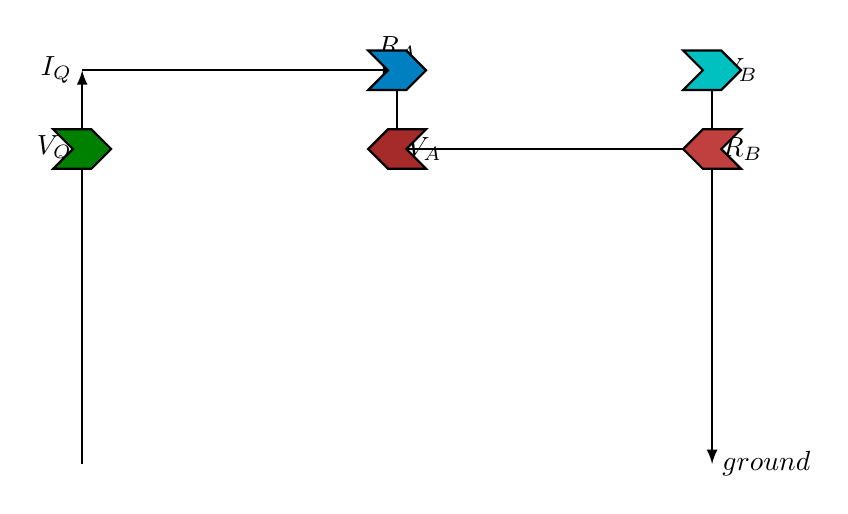
\begin{tikzpicture}[thick, >=latex]
    % Define colors
    \definecolor{myblue}{RGB}{0,128,192}
    \definecolor{myred}{RGB}{192,64,64}
    \definecolor{mygreen}{RGB}{0,128,0}
    \definecolor{mycyan}{RGB}{0,192,192}
    \definecolor{mybrown}{RGB}{165,42,42}
    \definecolor{mygray}{RGB}{128,128,128}

    % Draw the circuit
    \draw[->] (0,0) -- (0,4) node[left] {$V_Q$};
    \draw[->] (0,4) -- (0,5) node[left] {$I_Q$};
    \draw[->] (0,5) -- (4,5) node[above] {$R_A$};
    \draw[->] (4,5) -- (4,4) node[right] {$V_A$};
    \draw[->] (4,4) -- (8,4) node[right] {$R_B$};
    \draw[->] (8,4) -- (8,5) node[right] {$V_B$};
    \draw[->] (8,5) -- (8,0) node[right] {$\text{ground}$};

    % Add labels and annotations
    \node[draw, fill=mygreen, shape=signal, signal from=left, signal to=right, minimum width=0.5cm, minimum height=0.5cm] at (0,4) {};
    \node[draw, fill=myred, shape=signal, signal from=right, signal to=left, minimum width=0.5cm, minimum height=0.5cm] at (8,4) {};
    \node[draw, fill=myblue, shape=signal, signal from=left, signal to=right, minimum width=0.5cm, minimum height=0.5cm] at (4,5) {};
    \node[draw, fill=mybrown, shape=signal, signal from=right, signal to=left, minimum width=0.5cm, minimum height=0.5cm] at (4,4) {};
    \node[draw, fill=mycyan, shape=signal, signal from=left, signal to=right, minimum width=0.5cm, minimum height=0.5cm] at (8,5) {};
\end{tikzpicture}

\end{document}